%% Submissions for peer-review must enable line-numbering 
%% using the lineno option in the \documentclass command.
%%
%% Preprints and camera-ready submissions do not need 
%% line numbers, and should have this option removed.
%%
%% Please note that the line numbering option requires
%% version 1.1 or newer of the wlpeerj.cls file, and
%% the corresponding author info requires v1.2

%\documentclass[fleqn,10pt,lineno]{wlpeerj} % for journal submissions
\documentclass[fleqn,10pt]{wlpeerj} % for preprint submissions

%\newcommand{\rr}{${\mathcal{R}}$}
\usepackage{amssymb}
\usepackage{amsmath}
\usepackage{upgreek}
\usepackage[]{fontenc}
\usepackage{color}
\usepackage{bm}
\usepackage[english]{babel}
\usepackage{graphicx}
\usepackage{tikz}
\usetikzlibrary{positioning}
\usepackage{ifthen}
\usepackage{xstring}
\usepackage{afterpage}
%\usepackage[hidelinks]{hyperref}
\usepackage[colorlinks=true, allcolors=blue, pdfborder={0 0 0}]{hyperref}

\newcommand{\floor}[1]{\left \lfloor #1 \right \rfloor}
\newcommand{\round}[1]{\left \lfloor #1 \right \rceil }
\newcommand{\ceil}[1]{\left \lceil #1 \right \rceil }
\newcommand{\Fig}[1]{Fig.~\ref{#1}}
%\newcommand{\Fig}[1]{Figure~\ref{#1}}
\newcommand{\Figs}[1]{Figs.~\ref{#1}}
%\newcommand{\Figs}[1]{Figures~\ref{#1}}
\newcommand{\Sec}[1]{Section~\ref{#1}}
\newcommand{\Secs}[1]{Sections~\ref{#1}}
\newcommand{\Chap}[1]{Chapter~\ref{#1}}
\newcommand{\Chaps}[1]{Chapters~\ref{#1}}
\newcommand{\Tab}[1]{Table~\ref{#1}}
\newcommand{\Tabs}[1]{Tables~\ref{#1}}
\newcommand{\Eqn}[1]{Eqn.~\ref{#1}}
\newcommand{\Eqns}[1]{Eqns.~\ref{#1}}
\newcommand{\InEqn}[1]{Inequality~(\ref{#1})}
\newcommand{\InEqns}[1]{Inequalities~(\ref{#1})}
\newcommand{\Center}[1]{\textcolor{white}{.}\hfill#1\hfill\textcolor{white}{.}}
\newcommand{\ang}{$\textrm\AA$\xspace}
\newcommand{\new}[1]{#1}
\newcommand{\New}[1]{#1}
\newcommand{\n}[1]{#1}
\newcommand{\we}{I~}

\newcommand\solidrule[1][1cm]{\rule[0.5ex]{#1}{0.2mm}}
\newcommand\dotdashedrule{\mbox{%
  \solidrule[1.5mm]\hspace{0.75mm}\solidrule[0.2mm]\hspace{0.75mm}\solidrule[1.5mm]}}
\newcommand\dashedrule{\mbox{%
  \solidrule[1.5mm]\hspace{0.75mm}\solidrule[1.5mm]}}
\newcommand\dottedrule{\mbox{%
  \solidrule[0.2mm]\hspace{0.3mm}\solidrule[0.2mm]\hspace{0.3mm}\solidrule[0.2mm]\hspace{0.3mm}\solidrule[0.2mm]\hspace{0.3mm}\solidrule[0.2mm]\hspace{0.3mm}\solidrule[0.2mm]}}
  
  
\usepackage{xspace}

\newcommand{\pname}{\texttt{plotMAP}\xspace}
\newcommand{\code}[1]{\texttt{#1}\xspace}

\usepackage[cal=cm,scrscaled=1.05]{mathalfa} % This is for \mathcal{}, particularly \mathcal{R}
\DeclareMathAlphabet\mathbfcal{OMS}{cmsy}{b}{n} % for boldface mathcal: \mathbfcal{}
\newcommand{\rr}{$\mathcal{R}$\xspace}


\def\kt{k_{\rm B}T}


\def\beq{\begin{equation}}
\def\eeq{\end{equation}}
\def\bea{\begin{eqnarray}}
\def\eea{\end{eqnarray}}

\def\cal#1{\mathcal{#1}}
\def\eqq#1{Eq.~(\ref{#1})}
\def\eq#1{(\ref{#1})}
\def\av#1{\langle #1 \rangle}

\def\f#1{Fig.~\ref{#1}}
\def\ff#1{Figs.~\ref{#1}}

\def\s#1{Section~\ref{#1}}

\def\c#1{~\cite{#1}}


%\newcommand{\c}[1]{\citep{#1}}

\newcommand{\figdir}{./figures}

\title{Chirality and the Ramachandran plot}

\author[1,*]{Ranjan V. Mannige}
\author[1]{Other Names TBD}
%\author[1]{Ronald N. Zuckermann}
%\author[1]{Stephen Whitelam}
\affil[1]{~Molecular Foundry, Lawrence Berkeley National Laboratory, 1 Cyclotron Road, Berkeley, CA, U.S.A.}
\affil[*]{~rvmannige@lbl.gov}

% \keywords{Protein structure, Backbone Chirality, Backbone Twist}

\begin{abstract}
Proteins are a class of biomolecules that display diverse conformations, which is the reason for their diverse functionality. These conformations are afforded in large part due to a protein's `backbone', whose twists and contortions allow for a protein to fold into particular conformations. The Ramachandran plot has been used since the 1960's to describe the nature in which the backbone twists into regular structures\citep{Ramachandran1963}.  While the regions within the Ramachandran plot that are well-populated by proteins is well known, new molecules are being designed today that are not bound to the traditional regions of the Ramachandran plot. This has sparked new interest in the basic behavior of a backbone within all regions of the Ramachandran plot (not just those available to a canonical protein). In these lines, this short paper describes: 1) a complete characterization of the way a backbone twists in all regions of the Ramachandran plot -- this would serve as a reference point for understanding new types of peptide and peptidomimetic structures -- and 2) a succinct set of Python scripts that show how these types of studies are accessible to undergraduate students with basic computational and biological training.
\end{abstract}

\begin{document}

\flushbottom
\maketitle
\thispagestyle{empty}

\section*{Introduction}

%Proteins are a class of biomolecules unparalleled in their functionality \citep{Berg2006}. 

The Ramachandran plot \citep{Ramachandran1963} is a two-dimensional map that describes the per-residue conformation of a peptide backbone \citep{Berg2006,Alberts2002}. The Ramachandran plot is plotted as a function of a peptide residue's dihedral angles $\phi$ and $\psi$ (\Fig{fig:intro}a). Each point $(\phi,\psi)$ represents a `twist' of a peptide backbone in three-dimensional space. Any peptide built with uniform twist or backbone paramters (say, $\phi=X^\circ$ and $\psi=Y^\circ$) will result in a regular structure; some regular structures are thermodynamically stable and are called secondary structures (\Fig{fig:intro}b). These secondary structures pack together with the help of loops, which are also twisted \cite{Berg2006}. As such, Ramachandran plots have been useful for understanding a peptide backbone's general conformational state or `twistedness' at a glance \citep{Berg2006,Alberts2002,Subramanian2001,Laskowski1993,Hooft1997,Laskowski2003}. While the idea of a curved peptide backbone appears to be the domain of a mathematical puzzle or diversion, in practice, the curve of the peptide backbone completely defines the general structure of a protein: proteins are peptides whose backbones occupy specific conformations\footnote{These conformations can be specific folds in globular proteins or larger structural ensembles in intrinsically disordered proteins; \cite{Mannige2014b}.}. This is important because, in the molecular world, the conformations available to a protein (or any molecule) plays a large part in defining the possible functionalities available to that molecule \citep{Berg2006,Alberts2002}.


So far, our understanding the Ramachandran plot been limited to the secondary structures and loops posed by proteins \citep{Berman2000}. For example, structural biologists are aware that the negatively sloping diagonal (dashed line in \Fig{fig:intro}b; henseforth denoted as the `-ve diagonal') demarcates a change in backbone chirality. For example, the position of the idealized left- and right-handed $\upalpha$-helices (\Fig{fig:intro}c) -- respectively denoted as $\upalpha_\textrm{L}$ and $\upalpha$ in \Fig{fig:intro}b -- are on opposite sides of the the -ve diagonal\footnote{Note that left- and right-handed backbone twists are respectively associated with the L and D chiralities within the Fisher Projection system and S and R chiralities within the Cahn--Ingold--Prelog system \citep{Cross2013}.}. Additionally, the the $\upbeta$-strand exists predominantly on the right of the -ve diagonal, and their backbones are predominantly left-handed [see, e.g., discussions within \cite{Quiocho1977} and \cite{Shaw1977}\footnote{Note that a different metric for handedness in $\beta$ sheets exists today that addresses the handedness of a particular hydrogen bonding network and not the handedness of the participating peptide's backbone. See, e.g., \cite{Schulz1974} and \cite{Chothia1977}.}]. Indeed, all regular/ordered motifs within proteins that lie to the right (or top) of the -ve diagonal are left-handed in backbone twist; as a corolary, all ordered backbones to the left (or under) the -ve diagonal are right handed in nature (primarily, the $\upalpha$-, $\pi$- and $3_{10}$-helix; \Fig{fig:intro}b; $\pi$-helices are not shown due to low frequency in the protein databank). Na{\"i}vely, these observations lead to the hypothesis that the -ve diagonal of the Ramachandran plot separates the left handed backbones from the right handed backbones (\Fig{fig:intro}d). While even Pauling was cognizant of this general trend in peptide secondary structure [see, e.g., his notes on what is now known as the $\upalpha$-sheet; \cite{Pauling1951,Pauling1951a,Pauling1951b}], the picture in \Fig{fig:intro}d has so far remained an untested hypothesis.

While chirality or `twist' in regular protein secondary structures is well understood, peptide mimics -- especially pep\textit{toids} -- display new secondary structures that fall out of the regions regularly occupied by proteins. Peptoids are distinguished from peptides by the position of each sidechain on the backbone (\Fig{FigSIpeptoid}). Certain peptides display secondary structures in regions of Ramachandran plot that are not well characterized \citep{Sun2013,Goodman2007,Culf2010,Beke2006,Pohl2012,Zuckermann2009,Sun2013}. For example, a `higher-order' peptoid secondary structure -- the $\Sigma$-strand \citep{Mannige2015,Robertson2016} -- samples regions of the Ramachandran plot (`$\textrm{\textbf{I}}$' in \Fig{fig:intro}d) that are not permitted within natural proteins (this is because of the lack of backbone hydrogen bond donors in peptoids). Another secondary structure -- the `$\omega$-strand' \citep{Gorske2016} -- samples similarly `historically uncharted' regions of the Ramachandran plot (`$\textrm{\textbf{II}}$' in \Fig{fig:intro}d). Importantly, handedness plays a crucial part in explaining these new motifs: as one goes along the backbones of these secondary structures, alternating residues occupy equal but opposite backbone twists [for this reason, the $\sigma$ sheet is relatively linear, albeit meandering; \cite{Mannige2015}; \cite{MannigeKunduWhitelam2016}]. 

In light of these new secondary structures, and in anticipation of the discovery of additional (higher-order) secondary structures, we chose to test the hypothesis in \Fig{fig:intro}d. That is, we ask below: which way does the peptide/peptoid backbone twist at any point on the Ramachandran plot? This question, while simple, would complete our understanding of how twists combine to form structures.

\begin{figure}[t!]
\includegraphics[width=0.8\linewidth]{\figdir/chirality_intro.pdf}
\caption{\label{fig:intro} The general structures available to peptides and proteins are characterized the way in which the peptide backbone twists in three-dimensional space. }
\end{figure}

%In addition to a new class of peptide mimcs requiring a reassesment of the historically `less-traveled' regions of the Ramachandran plot: DISORDER.  Additionally, a number of proteins undergo conformational transitions, without which they may not properly function. Finally, some proteins -- intrinsically disordered proteins -- display massive disorder whose conformations dramatically change over time \citep{Uversky2003, Fink2005, Midic2009, Espinoza-Fonseca2009, Uversky2010, Tompa2011, Sibille2012, Kosol2013, Dunker2013, Geist2013, Mannige2014, Baruah2015}.

%Many of the useful/distinguishing structural properties of peptoids emerge from the primary feature that distinguishes peptoids from peptides: peptoid sidechains are attached to backbone nitrogen atoms rather than backbone $\upalpha$-carbon atoms (\Fig{FigSIpeptoid}). Interestingly, this change in the sidechain's position drastically alters the structural and dynamical properties of the peptoid backbone (e.g., protein secondary structure facilitating hydrogen bond donors are missing in peptoids\cite{Berg2006,Matsuurua2014}). These unique properties allow for peptoids of specific sequences to form a wide range of stable structures\cite{Paul2011,Butterfoss2012,Yoo2008,Shah2008,Laursen2013,Butterfoss2009,Nam2010}.
%Particularly relevant from a design perspective, some peptoids have been shown to display structures -- self-healing membrane-like peptoids\cite{Haibao2016} and peptoid nanosheets\cite{Nam2010,Sanii2011,Kudirka2011,Mannige2015} -- that are nanoscale in some dimensions and mescoscopic in other dimensions. Such atomistically intricate yet mesoscopic assemblies are unseen in natural proteins, and serve as proof-of-concepts for the further search for novel peptoid assemblies. However, unlike evolution's considerable sampling capabilities, the discovery of such novel peptoid structures and assemblies are limited to the speed at which chemists are able to design and produce such molecules. This limitation raises the utility of the high-throughput exploration of peptoid chemistry and structure with the help of computational simulation.

\section*{Methods}

In order to satisfy historical notation \citep{Berg2006,Alberts2002,Laskowski1993,Laskowski2003}, we assume $\phi$ and $\psi$ range between $-180^\circ$ and $180^\circ$\footnote{An angle $\zeta$ can be wrapped within the range $[-180,180)$ using $\zeta' = - 180 + (\zeta + 180) \% (360)$, where $\%$ represents the modulus function.}.

{\it Backbone twist handedness.} To explore the nature of backbone handedness, we use a metric that was previously used as a measure of helix twist handedness \citep{Kwiecinska2005}\footnote{With the exception of certain regions within the Ramachandran plot (e.g., $\phi=\psi=180^\circ$), all regularly arranged backbones are helices. Indeed, the word `helix' has a broad meaning that comes from the greek word $\check\epsilon\lambda\iota\xi$ that means `twisted, curved'; \cite{Liddell1894}.}:
\begin{equation} \label{chi1}
\chi_\textrm{b} = \frac{1}{N}\sum_{i = 2}^{N-2} \frac{(\textit{\textbf{v}}_{i-1} \times \textit{\textbf{v}}_{i})\cdot \textit{\textbf{v}}_{i+1}}{\textit{v}_{i-1} \textit{v}_{i} \textit{v}_{i+1}}.
\end{equation}
Here, $N$ is the peptide length, and the average peptide backbone handedness $\chi_\textrm{b}$ has range $[-1,1]$. Values deviating from 0 are more chiral (or `twisted' or `handed'), and left handed twists are negative while right handed twists are positive. Only $\upalpha$-carbon atom positions are used for the calculation. Each $\upalpha$-carbon belonging to residue $i \in \{ 1,2,\ldots N \}$ has position $\textit{\textbf{N}}_i$. %Vector $\textit{\textbf{v}}_{ij} \equiv \textit{\textbf{N}}_{i} - \textit{\textbf{N}}_{j}$ and $\textit{\textbf{v}}_{k} \equiv \textit{\textbf{v}}_{k+1,k} = \textit{\textbf{N}}_{k+1} - \textit{\textbf{N}}_{k}$. 
Vector $\textit{\textbf{v}}_{k} \equiv \textit{\textbf{N}}_{k+1} - \textit{\textbf{N}}_{k}$. 
The scalar component of the vector $\textit{\textbf{v}}_i$ is denoted as $\textit{v}_i$. Each scalar in the denominator within the summand (e.g. $\textit{v}_i$) indicates the distance between neighboring alpha carbons, which is $\sim$3\ang and $\sim$3.85\ang for backbones whose amide dihedral angles respectively are $cis$ ($\omega\approx0^\circ$) and $trans$ ($\omega\approx180^\circ$). If we know that the backbone amide is either all-$cis$ or all-$trans$, then the demnominator can be simplified to $\textit{v}_i^3$.

While we use this metric as the primary measure of handedness, we also use the following two metrics for reference:
\begin{equation}\label{chi2}
\displaystyle \chi_\textrm{b,2} = \frac{1}{\pi N}\sum_{i = 2}^{N-2}
 \textrm{arctan2}\left (\textit{v}_i \textit{\textbf{v}}_{i-1} \cdot \textit{\textbf{v}}_i \times \textit{\textbf{v}}_{i+1},\textit{\textbf{v}}_{i-1}\times \textit{\textbf{v}}_i \cdot \textit{\textbf{v}}_i\times \textit{\textbf{v}}_{i+1} \right ).
\end{equation}
%\begin{equation}\label{chi3}
%\displaystyle \chi_\textrm{b,2} = \frac{4!}{3N^4} \sum_{i,j,k,l \in \textit{\textbf{N}}} \frac{((\textit{\textbf{v}}_{ij} \times \textit{\textbf{v}}_{kl}) \cdot \textit{\textbf{v}}_{il}) (\textit{\textbf{v}}_{ij} \cdot \textit{\textbf{v}}_{jk}) (\textit{\textbf{v}}_{jk} \cdot \textit{\textbf{v}}_{kl})} {\left(\textit{v}_{ij} \textit{v}_{jk} \textit{v}_{kl}\right)^2 \textit{v}_{il}}.
%\end{equation}
$\chi_\textrm{b,2}$ is known as $\chi$ in \cite{Gruziel2013}, absent the normalization by $\pi$ used here to set the range from $-1$ to $1$ in stead of $-\pi$ to $\pi$. %$\chi_\textrm{b,2}$, of arbitrary range $[-\lambda,\lambda]$, is known as the chirality index $G_{0S}$ in \cite{Solymosi2002} and \cite{Neal2003}. $(i,j,k,l)$ are exhaustive permutations of $\{1,2,\ldots,N\}$.

{\it Generating regular peptides}
Peptides (poly-glycines; $N=5$) were generated using the Python-based PeptideBuilder library \citep{Matthew2013}. Analysis was performed using BioPython \citep{Cock2009} and Numerical Python \citep{Dubois1996}. Ramachandran plots that describe chirality (e.g., \Fig{fig:chi}a) were generated using a grid spacing of $\phi,\psi \in \{-180,-178,\ldots,178,180\}$.

{\it Protein secondary structure statistics.} $\upalpha$-helices, $3_{10}$-helices and $\beta$-sheets were identified using the DSSP algorithm \citep{Zhao2005,Kabsch1983,Joosten2011} and sourced from protein structures within the 40\% non-redundant database provided by the Structural Classification of Proteins or SCOP (Release 2.03; \cite{Fox2014}). The polyproline II helix statistics were obtained from segments within 16,535 proteins annotated by PolyprOnline \citep{Chebrek2014} to contain three or more residues of the secondary structure.

\section*{Results}

As depicted in \Fig{fig:intro}a, the backbone each residue $i$ of a peptide possesses two main degrees of freedom: the dihedral angles $\phi_i$,  and $\psi_i$. An additional degree of freedom exists, $\omega_i$, which in peptides predominantly occupies values of $\equiv180^\circ$ ($trans$), and infrequently occupies a lower-probability (higher-energy) value of $\equiv0^\circ$ ($cis$). \Fig{fig:chi} discusses the behavior of an all-$trans$ backbone, while \Fig{fig:chi_boundaries} describes the behavior of both all-$trans$ and all-$cis$ backbones. 

\Fig{fig:chi}a describes the twist or chirality ($\chi_\textrm{b}$; \Eqn{chi1}) of a regularly arranged backbone as a function of $(\phi,\psi)$ (additionally, an example of the behavior of one `slice' of \Fig{fig:chi}a is shown in \Fig{fig:chi}b). \Fig{fig:chi_boundaries}\textrm{(i)} and \Fig{fig:chi_boundaries}\textrm{(ii)} extends on \Fig{fig:chi} and describes the handedness of both $trans$ and $cis$ backbones in using two metrics ($\chi_\textrm{b}$,$\chi_\textrm{b,2}$). In each graph, negative (red) and positive (blue) values of handedness respectively indicate left- and right-handed backbone twists. The color white indicates that all $\upalpha$-carbon atoms in the conformation are coplanar. 

\begin{figure}[t!]
\includegraphics[width=0.9\linewidth]{\figdir/chi_snapshots.pdf}
\caption{\label{fig:chi} The chirality of an ordered peptide within the Ramachandran plot. Each point in (a) represents the chirality or handedness -- $\chi_\textrm{b}$ (\Eqn{chi1}) -- of a peptide backbone with uniform $(\phi,\psi)$  diehdral angles. 
Panel (a) shows that the na{\"i}ve expectation of handedness in a Ramachandran plot (\Fig{fig:intro}d) is too simplistic. Interestingly, our na{\"i}ve expectations (\Fig{fig:intro}d) would be upheld if we were only to have sampled regions of the Ramachandran plot dominated by known proteins (a; regions enclosed by `\protect\dottedrule'). An example of the behavior of one `slice' of (a) is shown in (b). The graph in \Fig{fig:chi}b represents the handedness of peptides (y-axis) whose backbones are built by setting $\phi_i=\psi_i=A$ ($A\in[-180^\circ,180^\circ]$). The graph is accompanied by snashots of peptides sampled at regions of the slice where $\chi_\textrm{b}$ is either 0 or at a local maximum or minimum. As expected, peptides whose carbon atoms are co-planar result in $\chi_\textrm{b}=0$.} %This is because, as expected, all regions allowed to a peptide that are to the left of the negative diagonal are right handed  and all corresponding regions to the right of the negative diagonal are left handed.}
\end{figure}

\begin{figure}[b!]
\includegraphics[width=0.8\linewidth]{\figdir/various_chis.pdf}
\caption{Panels (a) and (b) describe behavior of twists for backbones that are $trans$ ($\omega=180^\circ$) and $cis$ ($\omega=0^\circ$), respectively. Columns \textbf{\textit{(i)}} and \textbf{\textit{(ii)}} show, respectively, the behavior of the backbone as a measure of two metrics for twist handedness: $\chi_\textrm{b}$ (\Eqn{chi1}) and $\chi_\textrm{b,2}$ (\Eqn{chi2}) . Both plots show qualitatively identical apportionments of the Ramachandran plot into left and right handed twists. This general map is shown in column \textbf{\textit{(iii)}}.\label{fig:chi_boundaries}}
\end{figure}

\Figs{fig:chi} and~\ref{fig:chi_boundaries} assert the following: 1) the na{\"i}ve view of chirality (\Fig{fig:intro}d) is inaccurate for both the $trans$ (\Figs{fig:chi}a and~\ref{fig:chi_boundaries}\textit{a(i,ii)}) and $cis$ backbones (\Fig{fig:chi_boundaries}\textit{b(i,ii)}). For the $trans$ backbone, while the -ve diagonal (`\protect\dashedrule') does separate right($D$)- and left($L$)-handed backbone twists, it does not {\it exclusively} partition regions of oppossite handedness: two additional borders exist that also serve as $L$-$D$ demarcations (`\protect\dotdashedrule' in \Fig{fig:chi}). For the $cis$ backbone, the -ve diagonal does not even split the neighborhood into two parts: the -ve diagonal is adjacent to four regions of distinct handedness. 

In each Ramachandran plot within \Fig{fig:chi_boundaries}, both metrics for handedness -- $\chi_\textrm{b}$ \textit{(i)} and $\chi_\textrm{b,2}$\textit{(ii)} -- describe four regions of handedness, which are distinctly shaded in \textit{(iii)}. 

Interestinglyl, the reason for the na{\"i}ve view makes senses when considering only peptides: the -ve diagonal (`\protect\dashedrule') separates $D$ and $L$ twists if we consider only the regions occupied by structured proteins (`\protect\dottedrule' in \Figs{fig:chi}a and \ref{fig:chi_boundaries}a). 

Additionally, the -ve diagonal does not behave as mirror symmetry element\footnote{I.e., points on the Ramachandran plot that are related by a relection across the -ve diagonal do not code for backbones of opposing symmetry.}. In stead, the point $(0,0)$ serves as a two-fold point-group symmetry element with 

of one point on the ramachandran plot along the 

While this distribution of handedness within the Ramachandran plot deviates from the na{\"i}ve view (\Fig{fig:intro}d), the -ve diagonal nonetheless plays an important role: two points that are related by a reflection along the -ve diagonal also have their corresponding backbone structures related by mirror symmetry. 




regions are more 

In any frame of reference



While even Pauling was cognizant of this general trend in peptide secondary structure [see, e.g., his notes on what is now known as the $\upalpha$-sheet; \cite{Pauling1951,Pauling1951a,Pauling1951b}], the picture in \Fig{fig:intro}d has so far remained an untested hypothesis.





\begin{figure}[h!]
  \centering
  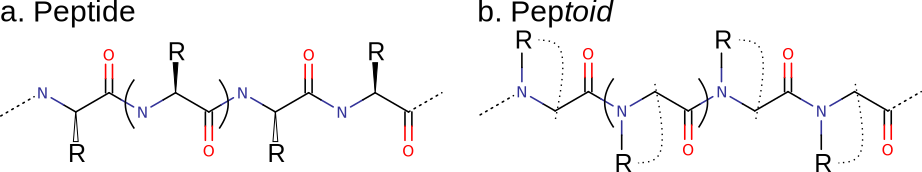
\includegraphics[width=0.9\textwidth]{\figdir/Figure_si_S1b.pdf}
  \caption{{\bf Peptoids and peptides are distinguished by the position of their sidechain (R) groups.} They therefore behave differently. For example, the peptoid backbone is more flexible than the protein one, and peptoid backbones lack canonical hydrogen bond donors, which are crucial to the formation of traditional secondary structures in proteins such as $\upalpha$-helices $\upbeta$-sheet \citep{Berg2006}.
\label{FigSIpeptoid}}
\includegraphics[width=\linewidth]{\figdir/various_chis_skewed.pdf}
\caption{\label{fig:other_chis_skewed} Each panel describes handedness data (right) and boundaries (left). While both frames of references $\left[-180^\circ,\ldots,180^\circ\right]$ (a,c) and $\left[0^\circ,\ldots,360^\circ\right]$ (b,d) yield similar trends for $trans$ backbones (a,b); however, for $cis$ backbones, the latter frame of reference (d) appears to more neatly apportion the behavior of backbone  than the traditional frame of reference (c).}
\end{figure}


\cite{Pauling1951a,Pauling1951}
\citep{MannigeKunduWhitelam2016}
ppI helix \citep{Adzhubei1993}


Backbones of natural amino acids with `L' chirality dominantly occupy the ``left side'' of the plot ($\phi<0$; \Fig{fig_altr}a, top), a consequence of the chirality of the backbone $\upalpha$-carbon \citep{Berg2006,Cintas2002} and steric hindrance between the backbone carbonyl and sidechain atoms (\cite{Branden1999}). Interestingly, switching the C$_\upalpha$'s chirality for every residue results in structures that exist on the ``other side'' of the plot, which a majority of its density at $\phi>0$; (\cite{Zawadzke1993,Hung1998}).


\section*{Acknowledgments}

RVM was supported by the Defense Threat Reduction Agency under contract no. IACRO-B0845281. RVM thanks Alana Canfield Mannige for her critique. This work was done at the Molecular Foundry at Lawrence Berkeley National Laboratory (LBNL), supported by the Office of Science, Office of Basic Energy Sciences, of the U.S. Department of Energy under Contract No. DE-AC02-05CH11231.

\bibliography{all}

\end{document}